\documentclass[border=10pt]{standalone}
\usepackage{pgfplots}
\pgfplotsset{compat=1.17}
\begin{document}
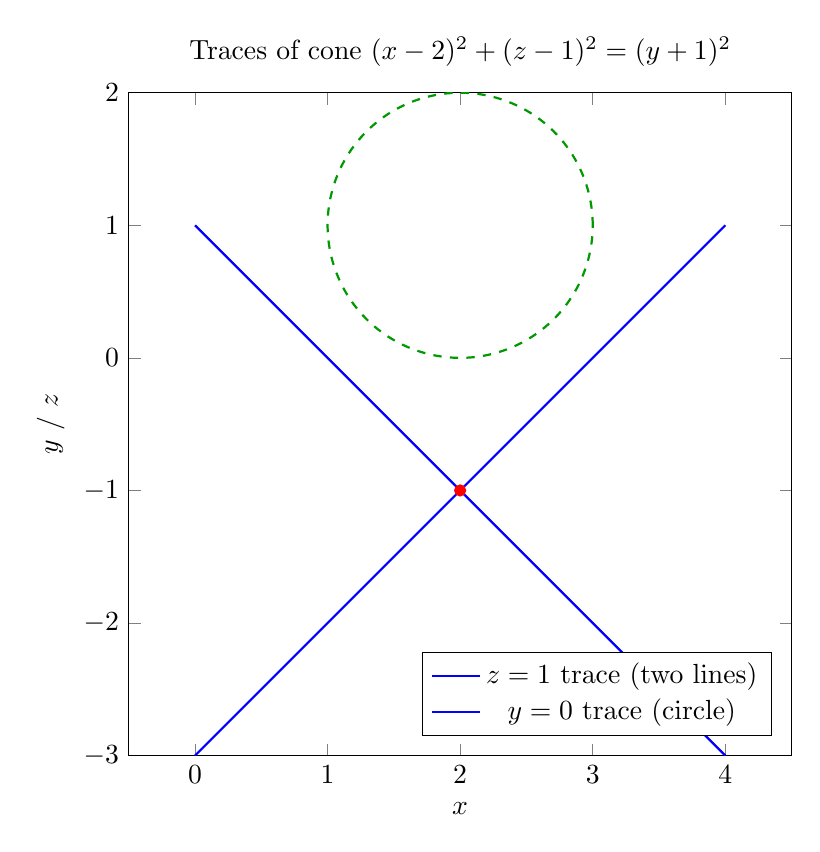
\begin{tikzpicture}
\begin{axis}[
    axis equal,
    xlabel={$x$}, ylabel={$y$ / $z$},
    xmin=0, xmax=4,
    ymin=-3, ymax=2,
    width=10cm, height=10cm,
    title={Traces of cone $(x-2)^2+(z-1)^2=(y+1)^2$},
    legend pos=south east,
]
\addplot[blue, thick, domain=0:4, samples=200] {x-3};
\addplot[blue, thick, domain=0:4, samples=200] {1-x};
\addlegendentry{$z=1$ trace (two lines)}
\addplot[green!60!black, dashed, thick, domain=0:360, samples=200] ({2+cos(x)}, {1+sin(x)});
\addlegendentry{$y=0$ trace (circle)}
\addplot[only marks, mark=*, red] coordinates {(2,-1)};
\end{axis}
\end{tikzpicture}
\end{document}
